Para medir los tiempos de ejecución de los algoritmos desarrollados, se utilizó la biblioteca \texttt{<chrono>} de C++, la cual permite capturar con alta precisión el intervalo de tiempo transcurrido entre el inicio y término de cada ejecución. Estas mediciones se realizaron automáticamente dentro del mismo programa, con el objetivo de garantizar consistencia y evitar interferencias externas.

\vspace{0.5 cm}

Los casos de prueba fueron generados automáticamente mediante un script en Python, el cual permite crear pares de cadenas de texto aleatorias con longitudes controladas. Estos casos se almacenan en archivos de texto ubicados en la carpeta \texttt{brute\_force\_input} y \texttt{dynamic\_programming\_input}, respectivamente, y son leídos por los programas en C++ al momento de ejecutar cada algoritmo.

\vspace{0.5 cm}

Durante la ejecución, los programas calculan la cantidad de substrings distintos entre las cadenas, y además registran el tiempo total de ejecución junto con la longitud promedio de los pares procesados. Posteriormente, se generaron gráficos a partir de estas mediciones utilizando scripts en Python, los cuales producen las visualizaciones correspondientes en la carpeta \texttt{plots} respectiva para cada parádigma.

\vspace{0.5 cm}

Este flujo garantiza la reproducibilidad de los experimentos, permitiendo observar que los resultados obtenidos reflejan fielmente el comportamiento real de los algoritmos. De este modo, fue posible comparar de forma objetiva el rendimiento de ambos enfoques en función del tamaño de entrada.

\vspace{0.5 cm}

\textbf{Algoritmo de fuerza bruta}

Para evaluar el rendimiento del algoritmo se generaron cuatro pares de cadenas idénticas en longitud para cada tamaño, desde 2 hasta 20 caracteres. Ese mismo caso se repitió sucesivamente para los diferentes tamaños. Los resultados de dichas mediciones se presentan en la tabla que sigue.

\begin{table}[H]
  \centering
  \footnotesize
  \begin{tabular}{@{}r S[table-format=1.6e1]@{}}
    \hline
    {$n$} & {Tiempo (s)} \\
    \hline
     2 & 5.708e-06 \\
     3 & 6.167e-06 \\
     4 & 1.8833e-05 \\
     5 & 1.8500e-05 \\
     6 & 4.5750e-05 \\
     7 & 1.13167e-04 \\
     8 & 4.61750e-04 \\
     9 & 1.33146e-03 \\
    10 & 5.09933e-03 \\
    11 & 1.82243e-02 \\
    12 & 5.98246e-02 \\
    13 & 1.76583e-01 \\
    14 & 6.32300e-01 \\
    15 & 2.27275e+00 \\
    16 & 1.10235e+01 \\
    17 & 3.71202e+01 \\
    18 & 1.61297e+02 \\
    19 & 5.58869e+02 \\
    20 & 2.54417e+03 \\
    \hline
  \end{tabular}
  \caption{Tiempos de ejecución para distintos largos $n$ de cadenas de texto.}
  \label{tab:tiemposDP}
\end{table}

El gráfico generado se presenta en la imagen que sigue.

\begin{figure}[H]
    \centering
    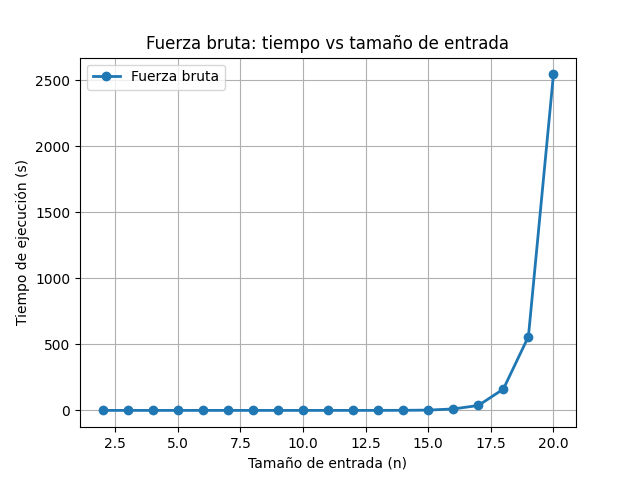
\includegraphics[width=0.8\textwidth]{code/brute_force/data/plots/brute_force_plot.png}
    \caption{Tiempos de ejecución para el algoritmo de fuerza bruta.}
    \label{fig:selectionsort}
\end{figure}

Los datos obtenidos para el algoritmo de fuerza bruta revelan con mucha claridad el carácter exponencial de su tiempo de ejecución. Si se observan los puntos correspondientes a tamaños de entrada entre $n=2$ y $n=10$, los tiempos permanecen en el orden de los microsegundos, de modo que la curva luce prácticamente plana. Una vez que uno supera el largo de $n=10$, la pendiente de la curva comienza a inclinarse. Para $n=10-15$ se empieza a percibir un incremento en tiempo de ejecución. A partir de $n=16$, el comportamiento del algoritmo y su tiempo de ejecución se multiplica exponencialmente alcanzando más de 2.500 segundos. Esta aceleración casi vertical en el gráfico refleja la complejidad teórica del algoritmo: al explorar todas las subsecuencias posibles de cada cadena, el trabajo efectivo se duplica con cada carácter adicional.

\vspace{0.5 cm}

El resultado práctico es una escalabilidad nula: el algoritmo solo resulta utilizable para entradas muy pequeñas. A partir de $n=15$ o más, se vuelve poco manejable. Esta complejidad teorica tan pobre justifica el paso a enfoques más sofisticados, como lo es la programación dinámica, que reduce el problema a complejidad cuadrática permitiendo procesar cadenas de longitudes mucho mayores.

\vspace{0.5 cm}

La tabla y el gráfico no solo corroboran la validez del algoritmo de fuerza bruta, sino que también ponen de manifiesto su inviabilidad práctica y la necesidad de técnicas de optimización para cualquier aplicación que involucre secuencias de tamaño moderado.

\vspace{0.5 cm}

\textbf{Algoritmo de programación dinámica}

Para evaluar el rendimiento del algoritmo se generaron cuatro pares de cadenas idénticas en longitud para cada tamaño, desde 2 hasta 20 caracteres. Ese mismo caso se repitió sucesivamente para los diferentes tamaños. Los resultados de dichas mediciones se presentan en la tabla que sigue.

\begin{table}[H]
  \centering
  \footnotesize
  \begin{tabular}{@{}r S[table-format=1.5e1]@{}}
    \hline
    {$n$} & {Tiempo (s)} \\
    \hline
     2  & 8.2500e-06 \\
     3  & 1.6917e-05 \\
     4  & 1.0084e-05 \\
     5  & 1.0750e-05 \\
     6  & 1.4709e-05 \\
     7  & 1.4875e-05 \\
     8  & 1.5125e-05 \\
     9  & 1.6750e-05 \\
    10  & 1.8750e-05 \\
    11  & 1.2042e-05 \\
    12  & 2.5667e-05 \\
    13  & 2.1333e-05 \\
    14  & 2.3875e-05 \\
    15  & 2.4416e-05 \\
    16  & 2.5209e-05 \\
    17  & 3.0000e-05 \\
    18  & 2.6917e-05 \\
    19  & 3.6292e-05 \\
    20  & 1.8500e-05 \\
    \hline
  \end{tabular}
  \caption{Tiempos de ejecución para programación dinámica (tamaño de entrada $n$)}
  \label{tab:tiemposDP}
\end{table}

El gráfico generado se presenta en la imagen que sigue.

\begin{figure}[H]
    \centering
    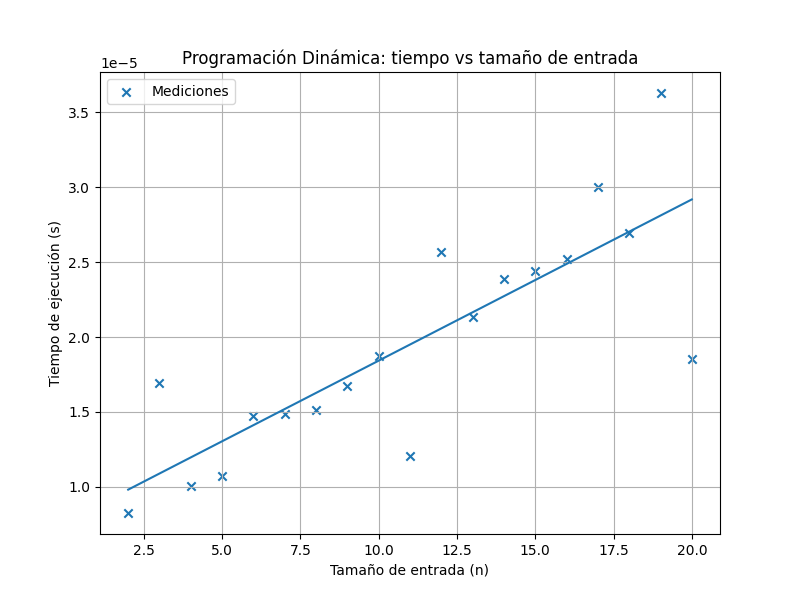
\includegraphics[width=0.8\textwidth]{code/dynamic_programming/data/plots/dynamic_programming_plot.png}
    \caption{Tiempos de ejecución para el algoritmo de programación dinámica.}
    \label{fig:selectionsort}
\end{figure}

Los datos obtenidos para el algoritmo de programación dinámica revelan con mucha claridad la eficiencia prevista para este enfoque. Todas las mediciones permanecen en el rango de los $10^{-5}$ segundos. En la práctica, el algoritmo es prácticamente instantáneo para cadenas de hasta veinte caracteres.

\vspace{0.5 cm}

El gráfico muestra que los puntos se agrupan en torno a una recta ascendente, lo que sugiere un crecimiento lineal dentro de los casos evaluados en la ejecución. Teóricamente, el algoritmo tiene complejidad cuadrática, pero con tamaños tan pequeños la parte cuadrática todavía no se vuelve dominante y la porción de la curva que alcanzamos a ver puede aproximarse razonablemente por una línea.

\vspace{0.5 cm}

Desde la perspectiva de la escalabilidad, la diferencia con la fuerza bruta es abismal. Aunque el algoritmo de programación dinámica necesita utilizar una matriz para su realización, el costo de llenarla es proporcional a $nm$ y, para los tamaños estudiados, se logran procesar en tiempos muy bajos.

\vspace{0.5 cm}

La tabla y el gráfico evidencian un algoritmo con rendimiento estable: su complejidad cuadrática no representa un obstáculo visible en este rango de entradas, y la ganancia frente a la solución de fuerza bruta justifica plenamente el uso de programación dinámica para calcular subsecuencias en aplicaciones reales.
